%\documentclass[13pt, oneside, a4paper, openany]{article}
\documentclass[14pt, oneside, a4paper, openany]{scrartcl}
\usepackage[utf8]{vietnam}
\usepackage{amsmath, amsbsy, amsxtra, latexsym, amssymb, inputenc, amsthm}
\usepackage[top=3.5cm, bottom=3cm, left=3.5cm, right=2cm]{geometry}
\usepackage{times}
\usepackage{graphicx}
\usepackage{systeme}
\usepackage{multirow}
\usepackage{imakeidx}
%\makeindex[options=-s index,columns=2,intoc=true]
\makeindex
\usepackage{indentfirst}
\setlength{\parindent}{1cm}
\usepackage{array}

\newtheorem{theorem}{Định lý}[section]
\newtheorem{corollary}{Hệ quả}[theorem]
\newtheorem{lemma}[theorem]{Bổ đề}
\newtheorem*{remark}{Chú ý}

%\usepackage{titlesec}
%\titleformat*{\section}{\LARGE\bfseries}
%\titleformat*{\subsection}{\Large\bfseries}
%\titleformat*{\subsubsection}{\large\bfseries}
%\titleformat*{\paragraph}{\large\bfseries}
%\titleformat*{\subparagraph}{\large\bfseries}

\usepackage{hyperref}

%\usepackage{sectsty}
%\sectionfont{\LARGE}
%\subsectionfont{\Large}
%\subsubsectionfont{\Large}
%\paragraphfont{\Large}

\usepackage{algorithm}
\usepackage[noend]{algpseudocode}

\algnewcommand\algorithmicinput{\textbf{Input:}}
\algnewcommand\INPUT{\item[\algorithmicinput]}

\algnewcommand\algorithmicoutput{\textbf{Output:}}
\algnewcommand\OUTPUT{\item[\algorithmicoutput]}

%\algnewcommand\algorithmicto{\textbf{to}}
%\algrenewtext{For}[3]%
%	{\algorithmicfor\ #1 \gets #2 \algorithmicto\ #3 \algorithmicdo}

\renewcommand{\listalgorithmname}{Danh sách thuật toán}

\usepackage{csvsimple}
\usepackage{relsize}

% first page
\linespread{1.25}
\let\circledS\undefined
\mathchardef\period=\mathcode`,
\newtheorem{example}{Ví dụ}[section]
\newtheorem{definition}{Định nghĩa}[section]
\mathchardef\period=\mathcode`,
\begin{document}

\thispagestyle{empty}

\centerline{\bf TRƯỜNG ĐẠI HỌC BÁCH KHOA HÀ NỘI}
\centerline{\bf VIỆN TOÁN ỨNG DỤNG \& TIN HỌC}
\centerline{\bf--------------------o0o--------------------}
\vspace*{1cm}
\begin{figure}[!ht]
\centering

\includegraphics[height=4cm,width=3cm]{anhbia.jpg} 
\end{figure}
\vspace*{1cm}

\centerline{\large\bf ỨNG DỤNG LÝ THUYẾT ĐỒ THỊ TRONG BÀI TOÁN THỰC TẾ}
\centerline{\large\bf Ứng dụng trong phân tích mạng giao thông và các đồ thị mạng xã hội}
\vspace*{1cm}
\centerline{\Large\bf ĐỒ ÁN TỐT NGHIỆP ĐẠI HỌC}
\centerline{\Large\bf Chuyên ngành: Toán Tin}
\vspace*{2cm}

\hspace{1.95cm} \textbf{Giáo viên hướng dẫn } 
\hspace{4mm} \textbf{:}
\textbf{\parbox[t]{10cm}{\hspace{0.85cm}LÊ CHÍ NGỌC}}

\hspace{2cm} \textbf{Sinh viên thực hiện }
\hspace{0.68cm} \textbf{:}
\textbf{\parbox[t]{10cm}{\hspace{0.85cm}NGÔ TRƯỜNG GIANG}}

\hspace*{1.95cm} \textbf{SHSV } 
\hspace{3.5cm} \textbf{:}
\hspace{10pt} \textbf{\parbox[t]{10cm}{\hspace{0.45cm}20121584}}
\vspace{2.5cm}
\vfill
\centerline{\bf Hà Nội - 06/2017}

\newpage
\thispagestyle{empty}
\centerline{\Large\bf NHẬN XÉT CỦA THẦY HƯỚNG DẪN}
\begin{enumerate}
	\item \textbf{Mục đích và nội dung của đồ án}
	\newline
	\newline
	\newline
	\newline
	\item \textbf{Kết quả đạt được}
	\newline
	\newline
	\newline
	\newline
	\item \textbf{Ý thức làm việc của sinh viên} \ldots
	\newline
	\newline
	\newline
	\newline
	\newline
	
	\begin{flushright}
		Hà Nội, ngày 07 tháng 05 năm 2017
	\end{flushright}
	\hspace{95 mm}Giảng viên hướng dẫn
	
	%\vspace*{2cm}
	\hspace{95 mm}(Ký và ghi rõ họ tên)
\end{enumerate}

%Create table of contents
\newpage
\thispagestyle{empty}
\tableofcontents
\newpage
% Create table of figures
\thispagestyle{empty}
\listoffigures
\listoftables
\listofalgorithms
\addtocontents{loa}{\def\string\figurename{Algorithm}}
\newpage
\section{Lời cảm ơn}
Lời đầu tiên, em xin chân thành cảm ơn các thầy giáo trong Trường Đại học Bách Khoa Hà Nội, cùng các thầy cô trong Viện Toán ứng dụng và Tin học, đã dành tâm huyết truyền đạt những kiến thức quý báu cho chúng em trong suốt những năm tháng học em tại trường.

Với lòng biết ơn sâu sắc, em xin cảm ơn thầy Lê Chí Ngọc đã giúp đỡ em rất nhiều trong quá trình thực hiện đồ án này.

Em cũng xin cảm ơn gia đình và bạn bè đã động viên, giúp đỡ em rất nhiều trong thời gian em làm đồ án.

Cuối cùng em xin chúc các thầy cô giáo trong Trường Đại Học Bách Khoa Hà Nội lời chúc sức khỏe và thành đạt.

\begin{flushright}
	Hà Nội, ngày 07 tháng 05 năm 2017
\end{flushright}
%\vspace*{2cm}
\hspace{95 mm}Ngô Trường Giang

\newpage
\section{Lời mở đầu}
%Những tiến bộ trong khoa học kĩ thuật trong những thâp kỷ gần đây đã cung cấp một lượng dữ liệu lớn về những mạng có kích thước lớn, có hàng triệu hoặc thậm trí hàng tỉ đỉnh như các mạng xã\
%Trong những thập kỉ gần đây, chúng ta đã chứng kiến sự bùng nổ của dữ liệu đồ thị nhờ có sự phát triển vượt bậc của internet và công nghệ thông tin. Ở dạng đơn giản nhất, đồ thị là một tập những đối tượng riêng biệt liên kết với nhau theo một cách nào đó. Những ví dụ về sự hiện diện của đồ thị có mặt ở khắp các lĩnh vực trong đời sống hiện đại, có thể kể đến ngay như mạng giao thông, mạng internet, mạng xã hội, mạng neuron, mạng tương tác protein, mạng lưới điện, và còn rất nhiều ví dụ khác nữa.\\
%Phân tích dữ liệu đồ thị là quá trình trích xuất những tri thức mới, có giá trị từ dữ liệu đồ thị, từ đó có thể đưa ra những quyết định tốt hơn. Chúng ta thường nhận ra sự quan trọng của phân tích dữ liệu đồ thị khi có sự bất thường trong những hệ thống được mô hình bằng đồ thị. Giống như khi một virus máy tính mới xuất hiện, chỉ trong một thời gian rất ngắn, có thể lan ra nhanh chóng trên Internet, và đánh sập hàng loạt những trang web quan trọng, đồng thời gây ra thiệt hại về bảo mật thông tin.\\
%Lúc đó, áp dụng đồ thị vào phân tích hệ thống có thể giúp phát hiện những hệ thống mạng đã bị ảnh hưởng, nhanh chóng cô lập và ngăn chặn sự lấy lan của virus.\\
%\cite{swissroad}
Phân tích dữ liệu đồ thị (graph analysis hoặc network analysis) là một lĩnh vực đang phát triển với mục đích khám phá ra những tri thức và hiểu biết về những dữ liệu được biểu diễn dưới dạng đồ thị.
Dữ liệu đồ thị có mặt khắp trong những lĩnh vực khác của đời sống hiện đại, từ mạng xã hội, mạng internet đến mạng giao thông, mạng lưới điện,...
Đồ thị thường được sử dụng để mô hình hóa dữ liệu khi liên kết, quan hệ giữa những đối tượng là trọng tâm của dữ liệu đó.
Ví dụ, trong khoa học xã hội, mỗi một node trong đồ thị tướng ứng với một người, và liên kết giữa những người đó có thể là quan hệ bạn bè nhưng trên Facebook, hay quan hệ đồng nghiệp như trên LinkedIn.
Trích xuất được những thông tin, tri thức mới từ những đồ thị này có thể thúc đẩy quá trình tìm kiếm công việc mới đối với người lao động và quá trình tuyển dụng nhân sự phù hợp của các công ty, như trên mạng xã hội công việc LinkedIn đã phát triển từ lâu.

Trong báo cáo này, tôi sẽ trình bày ứng dụng lý thyết đồ thị tìm tập độc lập cực đại trên giao thông và mạng xã hội cỡ lớn, một số kĩ thuật cơ bản trong phân tích dữ liệu đồ thị và áp dụng vào bài toán phân tích mạng giao thông đường bộ Việt Nam.

\newpage
\section{Giới thiệu}

\newpage
\section{Tập độc lập cực đại và các thuật toán heuristic tham lam}
\subsection{Các khái niệm cơ bản}
\begin{definition}
\cite{graphtextbook} Trong đồ thị đơn vô hướng $G = (V,E)$, một tập đỉnh con $S \subseteq V$ được gọi là \textbf{tập độc lập} \index{Tập độc lập} nếu không có hai đỉnh nào trong tập này kề nhau. Lực lượng của tập độc lập có kích thước lớn nhất được gọi là số độc lập của đồ thị, kí hiệu bởi $\alpha(G)$.	

Một tập độc lập được gọi là \textbf{tập độc lập cực đại} \index{Tập độc lập cực đại} nếu không tồn tại cách thêm một đỉnh trong $G$ vào tập này để thu được tập độc lập có lực lượng lớn hơn.

\textbf{Tập độc lập lớn nhất} \index{Tập độc lập lớn nhất} là tập độc lập có lực lượng (số đỉnh) lớn nhất trong tất cả các tập độc lập của đồ thị $G$.

\end{definition}
\begin{remark}
Tập độc lập lớn nhất thì là tập độc lập cực đại, nhưng tập độc lập cực đại chưa chắc đã là tập độc lập lớn nhất.	
\end{remark}

Bài toán tìm tập độc lập lớn nhất \index{Bài toán tìm tập độc lập lớn nhất} (MaxIS) được phát biểu như sau: cho đồ thị $G = (V,E)$, tìm tập độc lập trong $G$ có lực lượng lớn nhất.

Bài toán tìm tập độc lập cực đại \index{Bài toán tìm tập độc lập cực đại} (MIS) được phát biểu như sau: cho đồ thị $G = (V,E)$, tìm một tập độc lập cực đại trong $G$.


\begin{remark}
\cite{yannakakis01} Bài toán tìm tập độc lập lớn nhất trong đồ thị $G$ đã được chứng minh là bài toán NP-khó.
\end{remark}

Trong báo cáo này, tôi sẽ tập trung vào bài toán tìm tập độc lập cực đại (MIS), các thuật toán và ứng dụng của bài toán tìm tập độc lập cực đại trong thực tế. 

Một số ký hiệu được sử dụng:
\begin{itemize}
	\item Cho đồ thị $G = (V,E)$, ta kí hiệu $V(G)$ là tập đỉnh\index{tập đỉnh} của đồ thị và $E(G)$ là tập cạnh \index{tập cạnh} của đồ thị.
	\item $n(G) = |V(G)|$ là số đỉnh của đồ thị $G$, $m(G) = |E(G)|$ là số cạnh của đồ thị $G$. Nếu không nói gì thêm, ta viết tắt $V, E, n$ và $m$ lần lượt thay cho $V(G), E(G), n(G)$ và $m(G)$.
	\item Một cạnh (u,v) của đồ thị $G$ được kí hiệu là $uv$. Với $u,v \in V(G)$, ta kí hiệu $u \sim v$ nếu $uv \in E(G)$ và $u \nsim v$ nếu $uv \not\in E(G)$.
	\item Với mỗi đỉnh $u$ của đồ thị $G$, ta kí hiệu $N_G(u) = \{v \in V: uv \in E\}$ là tập đỉnh kề với đỉnh $u$, hay còn gọi là lân cận \index{lân cận} của $u$ trong đồ thị $G$.
	\item $\textrm{deg}(u)$ là bậc của đỉnh \index{bậc của đỉnh} $u$, trong đồ thị $G$, hay chính là số cạnh kề với cạnh $u$ trong đồ thị $G$.
	\item $\delta(G)$ là bậc nhỏ nhất \index{bậc nhỏ nhất} trong $G$, $\delta(G) := \min\{\textrm{deg}(u)\} , u \in V(G)$.
	\item $\Delta(G)$ là bậc lớn nhất \index{bậc lớn nhất} trong $G$, $\Delta(G) := \max\{\textrm{deg}(u)\} , u \in V(G)$.
	\item Ta kí hiệu đồ thị vòng  hay chu trình \index{chu trình} có $n$ đỉnh là $C_n$.
	\item Ta kí hiệu đồ thị đường hay đường đi \index{đường đi} có $n$ đỉnh là $P_n$.
	\item Ta kí hiệu đồ thị đầy đủ hai phía là $K_{m,n}$.
	%\item Đồ thị $(m,n)$-tadpole  \index{tadpole} là đồ thị đạt được bằng cách gắn một đồ thị chu trình $C_m$ với một đồ thị đường đi $P_n$ qua một cầu.
	\item \cite{graphclasses} Banner là đồ thị có dạng như hình 1.
	\begin{figure}[!h]
		\centering
		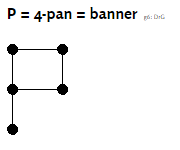
\includegraphics[scale=1]{figures/banner.png} 
		\caption[Đồ thị Banner]{Đồ thị Banner \cite{graphclasses}.}
	\end{figure}
\end{itemize}

Đồ thị $G'=(V',E')$ được gọi là đồ thị con của đồ thị $G=(V,E)$ nếu $V' \subset V$ và $E' \subset E$.

Ta gọi đồ thị $H$ là đồ thị con \textbf{cảm sinh} \index{cảm sinh} của đồ thị $G$ hay đồ thị $G$ cảm sinh $H$ nếu ta có thể thu được đồ thị $H$ băng cách xóa đi một số đỉnh trong đồ thị $G$ (có thể không xóa đi đỉnh nào) cùng với những cạnh kề với các đỉnh đó.

Một đồ thị con của $G$ cảm sinh bởi một tập đỉnh $U \subset V(G)$ là đồ thị thu được bằng việc xóa đi tất cả các đỉnh của tập đỉnh $V(G) \setminus U$ trong đồ thị $G$, kí hiệu đồ thị con này là $G[U]$.

Cho một tập đỉnh $W \subset V(G)$, ta cũng nói rằng $W$ cảm sinh đồ thị $H$ nếu $G[H]$ cảm sinh $H$.
\subsection{Alpha-redundant}
%Một đỉnh của đồ thị $G$ được gọi là $\alpha$-redundant nếu việc xóa đỉnh đó khỏi đồ thi $G$ không làm thay đổi số độc lập \index{số độc lập} của đồ thị $G$.
\begin{definition}
	\cite{alpharedundant} Cho đồ thị $G = (V,E)$, một đỉnh $v \in V(G)$ được gọi là $\alpha$-redundant \index{alpha-redundant} nếu $\alpha(G-v) = \alpha(G)$.
\end{definition}

Bài toán kiểm tra một đỉnh có phải là $\alpha$-redundant rõ ràng là tương đương với bài toán tìm tập độc lập cực đại, và đô đó thuộc lớp bài toán NP-complete. Tuy nhiên trong một số trường hợn, những đỉnh $\alpha$-redundant có thể nhận ra một cách hiệu quả.

\begin{lemma}
	\cite{alpharedudant2} Cho một đồ thị $G$ cảm sinh $K_{1,m}, \{u,v_1,v_2,...,v_m\}$, trong đó $u$ là đỉnh trung tâm (đỉnh có bậc $m$), sẽ tồn tại một số đỉnh $u_1,u_2,...,u_m$ sao cho $\{u,u_1,u_2,...,u_m\}$ là một tập độc lập và tồn tại một cặp ghép hoàn hảo giữa $\{u_i\}$ và $\{v_i\}$ hoặc $u$ là một đỉnh $\alpha$-redundant.
\end{lemma}

\subsection{Các thuật toán heuristic tham lam giải bài toán tìm tập độc lập cực đại}
Phương pháp heuristic có thể được sử dụng để tìm tập độc lập cực đại trong thời gian đa thức. Tôi sẽ tập trung vào những thuật toán heuristic tham lam để giải bài toán tìm tập độc lập cực đại.
%Tôi cũng sẽ đánh giá một số tính chất của những thuật toán này.

\subsubsection{Các phương pháp cổ điển}
Ta xem xét 3 thuật toán heuristic phổ biến cho bài toán tìm tập độc lập cực đại: MIN, MAX và VO (Vertex Ordering).

\paragraph{Thuật toán MIN}
Thuật toán MIN \index{MIN} được mô tả như sau: bắt đầu với một tập độc lập rỗng $I$, thuật toán liên tiếp chọn những đỉnh có bậc nhỏ nhất trong $G$, thêm đỉnh này vào tập $I$ và xóa đỉnh đó đi khỏi đồ thị $G$. Thuật toán dừng khi đồ thị $G$ không còn có đỉnh nào.

%%%%%%%%%%%%%%%
\begin{algorithm}
	\caption{MIN($G$)}\label{MIN}
	\begin{algorithmic}[1]
		\INPUT Đồ thị $G$
		\OUTPUT Một tập độc lập cực đại của G.
		\State $I:= \emptyset$; $i:=1$; $H_i := G$;
		\While{$V(H_i) \neq \emptyset$}
			\State Chọn $u \in V(H_i)$ sao cho $\textrm{deg}_{H_i}(u) = \delta(H_i)$;
			\State $I := I \cup \{u\}$; $i:=i+1$; $H_i := H_{i-1} - N_{H_{i-1}}[u]$;
		\EndWhile
		\State \textbf{end while}
		\State \textbf{return} $I$
	\end{algorithmic}
\end{algorithm}
%%%%%%%%%%%%%%%
\paragraph{Thuật toán MAX}
Trong thuật toán MAX \index{MAX} [3], ta liên tiếp lựa chọn một đỉnh có bậc lớn nhất trong đồ thị $G$, xóa đỉnh đó khỏi $G$ cho đến khi $G$ không còn có cạnh nào nữa. Những đỉnh còn lại hình thành một tập độc lập cực đại.

%%%%%%%%%%%%%%%
\begin{algorithm}
	\caption{MAX($G$)}\label{MAX}
	\begin{algorithmic}[1]
		\INPUT Đồ thị $G$
		\OUTPUT Một tập độc lập cực đại của G.
		\State $i:=n$; $H_i := G$;
		\While{$E(H_i) \neq \emptyset$}
			\State Chọn $u \in V(H_i)$ sao cho $\textrm{deg}_{H_i}(u) = \Delta(H_i)$;
			\State $i:=i - 1$; $H_i := H_{i+1} - u$;
		\EndWhile
		\State \textbf{end while}
		\State \textbf{return} $V(H_i)$
	\end{algorithmic}
\end{algorithm}
%%%%%%%%%%%%%%%
\paragraph{Thuật toán VO (Vertex Order)}
Trong thuật toán VO \index{VO} [4], đầu tiên ta xắp xếp các đỉnh của đồ thị $G$ theo thứ tự tăng về bậc của đỉnh. Sau đó lần lượt xử lý các đỉnh trong danh sách đã được xắp xếp và thêm đỉnh vào tập độc lập nếu nó không kề với bất cứ đỉnh nào trong tập độc lập hiện tại.

%%%%%%%%%%%%%%%
\begin{algorithm}
	\caption{VO($G$)}\label{VO}
	\begin{algorithmic}[1]
		\INPUT Đồ thị $G$
		\OUTPUT Một tập độc lập cực đại của G.
		\State $I := \emptyset$;
		\State Sắp xếp tập đỉnh V(G) thành một danh sách tăng dần về bậc của đỉnh ($u_i$);
		\For {i:=1 \textbf{to} $n(G)$}
			\If {$N_I(u_i) = \emptyset$}
				\State $I:= I \cup \{u_i\}$;
			\EndIf
			\State \textbf{end if}					
		\EndFor
		\State \textbf{end for}
		\State \textbf{return} $I$
	\end{algorithmic}
\end{algorithm}
%%%%%%%%%%%%%%%

%\subsubsection{Cận Caro-Wei}
%Cho đồ thị $G$, ta kí hiệu $k_{MIN}(G)$, $k_{MAX}(G)$, và $k_{VO}(G)$ là lực lượng nhỏ nhất của tập độc lập cực đại đại được bằng thuật toán MIN, MAX, và VO. Wei[5] đã sử dụng thuật toán MIN để tìm ra cận dưới của $\alpha(G)$:
%$$
%\alpha(G) \geq k_{MIN}(G) \geq \sum_{v \in V(G)} \frac{1}{\textrm{deg}(v)+1}
%$$
%Caro[6] cũng độc lập chứng minh kết quả này. Griggs[3] cũng chỉ ra rằng thuật toán MAX có thể được sử dụng để chứng minh cận Caro-Wei.
%Ngoc C. Le et al.[2] đã chứng minh được một kết quả cho thuật toán VO:
%$$
%k_{VO}(G) \geq \sum_{v \in V(G)} \frac{1}{deg(v)+1}
%$$

\subsubsection{Phương pháp kết hợp}
Trong phần này, tôi sẽ mô tả một phiên bản được chỉnh sửa của thuật toán heuristic tham lam cổ điển. Thuật toán là sự kết hợp của thuật toán MIN và 
$\alpha$-redundance, được đề xuất bởi Ngoc C. Le et al. \cite{MIS}.
Ta có hệ quả sau rút ra từ bổ đề 4.1 trong trường hợp $m=2$.
\begin{corollary}
	Cho đồ thị $G = (V,E)$, một đỉnh $u \in V(G)$ là $\alpha$-redundant nếu tồn tại hai đỉnh $v_1, v_2 \in N(u)$ sao cho $v_1 \nsim v_2$ và không tồn tại hai đỉnh $u_1, u_2$ sao cho $\{u,u_1,u_2\}$ là độc lập và $\{u,u_1,u_2,v_1,v_2\}$ cảm sinh $K_{2,3}$ hoặc banner hoặc $P_5$.
\end{corollary}

Thuật toán NMIN \index{NMIN} là sự kết hợp của kĩ thuật $\alpha$-redundant và thuật toán MIN.

Cho $G$ là một đồ thị đơn,vô hướng bất kỳ, gọi $n = |V(G)|$. Thuật toán NMIN trả về một tập độc lập cực đại. Thuật toán liên tiếp lựa chọn một đỉnh có bậc nhỏ nhất là $u$, sau đó kiểm tra và xóa đỉnh $u$ nếu $u$ là $\alpha$-redundant bằng cách áp dụng hệ quả 4.0.1.


%%%%%%%%%%%%%%%
\begin{algorithm}
	%\algsetup{linenosize=\Large}
	\caption{NMIN($G$)}\label{NMIN}
	\begin{algorithmic}[1]
		\INPUT Đồ thị $G$
		\OUTPUT Một tập độc lập cực đại của G.
		\State $I := \emptyset$; $i:=1$; $H_i=G$;
		\While {$V(H_i) \neq \emptyset$}
		\State Chọn $u \in V(H_i)$  sao cho $deg_{H_i}(u) = \delta(H_i)$;
		\ForAll {$v_1,v_2 \in N_{H_i}(u)$ sao cho $v_1 \nsim v_2$}
			\If {Không tồn tại $u_1,u_2 \in V(H_i)$ sao cho $\{u,u_1,u_2\}$ là độc lập và $\{u,u_1,u_2,v_1,v_2\}$ cảm sinh $P_5$ hoặc banner hoặc $K_{2,3}$}
				\State $H_{i+1} := H_i - u$; $i := i+1$; \textbf{Break};
			\EndIf
			\State \textbf{end if}
		\EndFor
		\State \textbf{end for}				
		\State $I := I \cup {u}$; $i := i+1$; $H_i := H_{i-1} - N_{i-1}[u]$;
		\EndWhile
	\State \textbf{end while}
	\State \textbf{return} $I$
	\end{algorithmic}
\end{algorithm}
%%%%%%%%%%%%%%%
%Cho một đồ thị đơn vô hướng bất kì $G$, gọi $n = |V(G)|$ thì thuật toán NMIN cho ra một tập độc lập cực đại. Ta có thể tìm ra đỉnh có bậc nhỏ nhất trong $G$ trong thời gian $O(n^2)$. Cho $(v_1,u,v_2)$ cảm sinh $P_3$, ta có thể kiểm tra liệu có tồn tại hai đỉnh $u_1, u_2$ sao cho $(u, u_1,u_2)$ là độc lập và $\{u,u_1,u_2,v_1,v_2\}$ cảm sinh $K_{2,3}$, banner, hoặc $P_5$ trong thời gian $O(n^2)$.

%Bài toán tìm tập độc lập có lực lượng hớn nhất và tính toán số độc lập của đồ thị có những ý nghĩa quan trọng trong nhiều lĩnh vực của đới sống, như lý thyết thông tin, sinh học, quản lý giao thông, viễn thông, v.v.\\
%Đầu tiên ta sẽ nhắc lại một số khái niệm cơ bản về lý thuyết đồ thị và tập độc lập, những định lý liên quan đến tập độc lập cực đại, và một số ứng dụng của bài toán tìm tập độc lập cực đại.

\newpage
\section{Ứng dụng của tập độc lập cực đại trong dịch tễ học}
\subsection{Giới thiệu về dịch tễ học}
Theo Bonita R, Beaglehole R, Kjellstrom K.\cite{BasicEpid}, \textbf{dịch tễ học}  \index{dịch tễ học} là khoa học nền tảng của y tế công cộng, được định nghĩa là "việc nghiên cứu sự phân bố của các yếu tố quyết định của các tình trạng hay sự kiện liên quan đến sức khỏe trong các quần thể xác định và việc ứng dụng những nghiên cứu này vào phòng ngừa và kiểm soát các vấn đề sức khỏe". 

Các nhà dịch tễ học không chỉ quan tâm đến tử vong, bệnh tật mà còn tới cả trình trạng sức khỏe và quan trọng nhất là giải pháp tăng cường sức khỏe cho cộng đồng.

Trọng tâm của các nghiên cứu dịch tễ học là các quần thể xác định về địa lý hoặc các khía cạnh khác. Một quần thể dược đề cập trong dịch tễ học thường là quần thể được chọn từ một khu vực đặc thù hay một nước vào một thời điểm cụ thể. Cấu trúc của các quần thể khác nhau ở các vùng địa lý khác nhau ở các thời điểm khác nhau có thể rất khác nhau. Nghiên cứu dịch tễ học rất quan tâm đến sự giao động này.

Dịch tễ học cùng với các thành tựu trong y học đã đạt được nhiều thành tựu không chỉ trong nghiên cứu mà còn trong thực tế, với những đóng góp lớn trong thanh toán các bệnh dịch lớn cũng nhưng phát hiện nguyên nhân của nhiều căn bệnh trong xã hội. 
Một trong những thành tựu phải kể đến là việc phát hiện ra rằng nhiễm khuẩn đậu bò sẽ góp phần bảo vệ chống virut đậu mùa, hay tìm ra nguyên nhân gây ra bệnh Minamata tại Nhật Bản là do ô nhiễm môi trường gây nhiễm độc Methyl thủy ngân.

\subsection{Dịch tễ học và lý thuyết đồ thị}
Đồ thị (hay mạng) và dịch tễ học về các bệnh truyền nhiễm có mối liên kết chặt chẽ với nhau. Nền tảng của dịch tễ học và những mô hình dịch tễ dựa trên sự phân bố ngẫu nhiên của quần thể, nhưng trong thực tế, mỗi cá thể trong quần thể có quan hệ với một tập những cá thể khác mà cá thể này có thể lây nhiễm hoặc bị lây nhiễm bệnh. Kết hợp tất các các mối quan hệ này, coi mỗi cá thể là một đỉnh của đồ thị và các quan hệ là các cạnh giữa các đỉnh cho ta một mạng truyền nhiễm của quần thể.

Những kiến thức về cấu trúc của mạng truyền nhiễm cho phép tính toán những chỉ số trong mô hình dịch tễ học từ hành vi lây nhiễm của những cá thể. Do đó, những đặc tính của mạng truyền nhiễm trở nên quan trọng trong củng cố những hiểu biết và dự đoán về các mô thức truyền nghiễm và đo lường tác động của những can thiệp vào quần thể.

\subsection{Bài toán tìm tập độc lập cực đại và ứng dụng trong dịch tễ học}

Một trong những quan tâm của dịch tễ học là làm sao tiêm phòng cho một nhóm cá thể với số lượng ít nhất có thể trong quần thể, nhằm ngăn chặn sự lan rộng của bệnh truyền nhiễm, như ta có thể tham khảo trong hình 2.

\begin{figure}[!h]
	\centering
	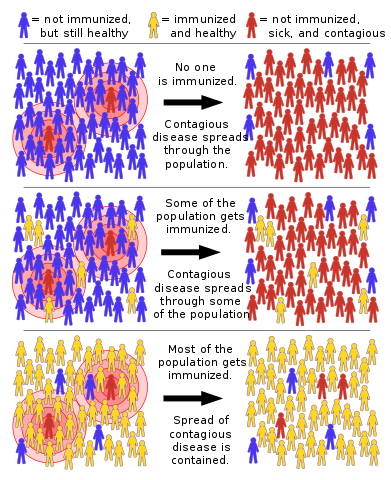
\includegraphics[scale=0.7]{figures/Herd_immunity.png} 
	\caption[Mô tả tác động của việc tiêm phòng đến sự truyền nhiễm của bệnh dịch]{Mô tả tác động của việc tiêm phòng đến sự truyền nhiễm của bệnh dịch (nguồn \href{https://en.wikipedia.org/wiki/Herd\_immunity}{Wikipedia}). Ta nhận thấy khi trong cộng đồng không có người được tiêm phòng (miễn nhiềm với bệnh dịch) thì bệnh dịch sẽ lan ra tự do. Khi chỉ có một số lượng nhỏ người được tiêm phòng cũng không ngăn được sự lan ra của bệnh dịch. Chỉ khi phần lớn cộng đồng được tiêm phòng, thì sự lan truyền của bệnh dịch mới được ngăn chặn.}
\end{figure}

Dưới góc độ dịch tễ học, một cá thể đã tiêm phòng (miễn nhiễm với bệnh dịch) sẽ khó có thể bị mắc lại và cũng không thể trở thành cá thể trung gian lan truyền bệnh cho những cá thể khác được. 

Còn dưới góc độ của lý thuyết đồ thị, như đã đề cập trong phần 4.1, một tập đỉnh của đồ thị không có hai đỉnh nào kề nhau thì tập đỉnh này được gọi là tập độc lập. 

Vì vậy, nếu tìm được một tập những cá thể không có liên hệ trực tiếp với nhau trong mang truyền nhiễm của quần thể (tập độc lập), ta chỉ cần tiêm phòng cho những cá thể còn lại của quần thể, thì kết quả là ta cô lập được những cá thể của tập cá thể không có liên hệ trực tiếp, để họ không thể truyền nhiễm lẫn nhau được nữa và bệnh dịch được giải quyết.

Yêu cầu đặt ra có thể là tập cá thể không có quan hệ trực tiếp này phải chứa tất cả các cá thể đã, đang và có thể bị bệnh của quần thể (chưa được miễn dịch). Để giảm thiểu số cá thể phải tiêm phòng nhằm giảm chi phí cho xử lý bệnh dịch, ta cần cực đại hóa tập cá thẻ không có quan hệ trực tiếp trên, tức là quay trở về bài toán tìm tập độc lập cực đại trong đồ thị.
Đây chính là một ứng dụng đơn giản của lý thuyết đồ thị trong dịch tễ học.

\subsection{Kết quả các thuật toán tìm tập độc lập cực đại trên các đồ thị cỡ lớn}
Sau đây tôi sẽ trình bày kết quả thực hiện các thuật toán tìm tập độc lập đã đề cập trong phần 4.3 (bảng 1), trên các bộ dữ liệu mạng cỡ lớn, và đánh giá kết quả của các thuật toán.

\begin{table}[!h]
	\caption[độ chính xác của các phương pháp trên các dữ liệu kiểm thử]{Kết quả chạy các thuật toán tìm tập độc lập cực đại với các dữ liệu đường bộ của các thành phố trên thế giới. Cột thứ nhất là tên thành phố, cột thứ hai và thứ ba lần lượt là số đỉnh và số cạnh của đồ thị. Các cột còn lại là kích thước của tập độc lập tìm được ứng với mỗi thuật toán.}
	\centering
	\csvautotabular{MIS.csv}
\end{table}

\subsection{Nhận xét kết quả}
Từ kết quả chạy thuật toán trong bảng 1, ta có thể thấy kích thước của tập độc lập thu được là khá lớn so với kích thước của đồ thị, suy ra tập đỉnh còn lại cần phản "tiêm phòng" khá nhỏ để đạt được hiệu quả ngăn chặn bệnh dịch lây lan ra cộng đồng.

\newpage
\section{Ứng dụng lý thuyết đồ thị trong phân tích mạng giao thông Việt Nam}
Theo Wikipedia, \textbf{giao thông vận tải} \index{giao thông vận tải} là quá trình dịch chuyển của con người, động vật và hàng hóa từ nơi này đến nơi khác. Những loại hình giao thông vận tải gồm có: đường không, đường sắt, đường bộ, đường thủy, đường ống, dây cáp và ngoài không gian (vũ trụ). Những yếu tố cơ bản trong hệ thống thông vận tải bao gồm: \textbf{cơ sở hạ tầng}, \textbf{phương tiện} và \textbf{vận hành}. Giao thông vận tải rất quan trọng vì nó cho phép sự trao đổi qua lại giữa con người, vốn là nguồn gốc sự phát triển của nền văn minh.

Cơ sở hạ tầng giao thông vận tải bao gồm sự xây dựng cố định của các loại đường đi như đường bộ, đường sắt, đường thủy, đường ống,... và các địa điểm đầu cuối như sân bay, nhà ga, kho hàng, cảng biển,... Những địa điểm đầu cuối có thể được sử dụng như nơi trung gian vận chuyển con người và hàng hóa hoặc là nơi lưu trữ.

Phương tiện di chuyển ở trong giao thông vận tải rất đa dạng, từ đơn giản như đi bộ, phổ biến như xe ôtô, cho đến hiện đại như máy bay hay tàu vũ trụ.

Vận hành hệ thống giao thông vận tải liên quan đến cách các phương tiện tham gia giao thông được điều khiển, liên quan đến những vấn đề khác như luật pháp, tài chính và các quy định. Trong ngành công nghiệp giao thông vận tải, cơ sở hạ tầng giao thông có thể được xây dựng để phục vụ mục đích công cộng hoặc do một tổ chức tư nhân đứng ra xây dựng và vận hành.

Giao thông vận tải có vai trò rất quan trọng đối với mọi mặt của xã hội hiện đại, khả năng mô hình hóa được mạng lưới giao thông, đưa ra được những phân tích và đánh giá về trình trạng của hệ thống giao thông có ý nghĩa rất quan trọng, hỗ trợ quá trình đưa ra quyết định chính xác, cho những nhà quản lý hệ thống giao thông, những công ty về dịch vụ giao thông vận tải, những nhà quy hoạch xây dựng và đất đai, và tất cả các đối tượng đang sử dụng hệ thống giao thông.

Trong phần này của báo cáo, tôi sẽ trình bày quá trình xây dựng mô hình đồ thị cho mạng giao thông quốc lộ của Việt Nam, với nguồn là dữ liệu GIS về các đường quốc lộ. Từ mô hình đồ thị, tôi đo lường một số chỉ số về độ phân cụm của mạng, độ trung tâm của những nút trong mạng, tính hiệu quả của mạng, từ đó đưa ra phân tích về tình trạng giao thông tại Việt Nam.

%\subsubsection{Cung và cầu của hệ thống giao thông vận tải}
%Mỗi một \textbf{nhu cầu vận chuyển} trong hệ thống giao thông vận tải đều là để phục vụ một nhu cầu nào đó khác ngoài đơn thuần là sự dịch chuyển. Hệ thống giao thông vận tải thực chất là hệ thống dịch vụ, và dịch vụ vận chuyển qua này sẽ phụ thuộc vào khả năng phục vụ của cơ sở hạ tầng giao thông, hay chính là khả năng \textbf{cung cấp dịch vụ} của hệ thống giao thông.
%
%Mọi nền kinh tế đều bao gồm các hoạt động diễn ra ở những địa điểm khác nhau, và sự dịch chuyển trao đổi phải diễn ra trong hệ thống giao thông vận tải. Nếu không có sự dịch chuyển thì hệ thống giao thông vận tải sẽ không có ý nghĩa và nếu không có giao thông vận tải thì sự dịch chuyển không thể xảy ra. Mối quan hệ phụ thuộc qua lại này có thể được nhìn nhận như một quan hệ cung-cầu trong kinh tế học, nhưng áp dụng đối với giao thông vận tải.
%
%Cung nhau khả năng cung cấp dịch vụ vận tải, là khả năng phục vụ của hệ thống cơ sở hạ tầng giao thông. Cung của hệ thống giao thông vận tải có thể được biểu diễn như 
\subsection{GIS}
Khái niệm GIS thường được hiểu là viết tắt của Geographical Information System, tức hệ thống thông tin địa lý, là một hệ thống máy tính, lưu trữ, xử lý và hiển thị dữ liệu địa lý.
GIS cũng có thể được hiểu là Geographical Information Sciences, tức khoa học về thông tin địa lý, được sử dụng bởi các hệ thống thông tin địa lý. Trong cáo cáo này, GIS được mặc định là viết tắt của khoa học thông tin địa lý.
\subsubsection{Các khái niệm cơ bản trong GIS}
Vị trí (location) trong GIS thể hiện những điểm trên bề mặt của trái đát. Cách thông thường trong đo lường vị trí trên trái đất là sử dụng hệ tọa độ kinh độ vĩ độ.

Khoảng cách (distance) trong GIS có nhiều loại khác nhau, có khoảng cách góc, khoảng cách tuyến tính hay khoảng cách theo đường chim bay và khoảng cách đường đi. Mỗi một loại khoảng cách lại có đơn vị đo khác nhau và được sử dụng vào một mục đích khác nhau.

Phép chiếu (projection) là một biến đổi toán học, giúp tạo ra bản đồ hai chiều của trái đất từ không gian ba chiều. Những phép chiếu nổi tiếng: phép chiếu Mercator, phép chiếu UTM.
Có hàng trăm phép chiếu khác nhau được phát triển, và không có phép chiếu nào là hoàn hảo, luôn có sự sai lệch trong biểu diễn bản đồ. Một số bản đồ giúp bảo toàn diện tích nhưng lại làm biến dạng hình dạng của đối tượng địa lý, ngược lại có những bản đồ bảo toàn hình dạng của đối tượng địa lý nhưng lại sai về diện tích.

Hệ tọa độ địa lý (coordinate system) cho phép biểu diễn vị trí của các điểm trên trái đất trong một hệ tọa độ, thường liên quan đến phép chiếu và các quy định về kích thước và hình dạng của trái đất. Một hệ tọa độ địa lý thường dduocjw sử dụng là UTM (Universal Transverse Mercator), chia thế giới thành 60 vùng khác nhau, mỗi vùng có một phép chiếu khác nhau để làm giảm sai lệch của phép chiếu.

Trong GIS, để biểu diễn các đối tượng địa lý trên bản đồ, người ta sử dụng khái niệm hình dạng. Có ba loại hình dạng cơ bản được sử dụng, đó là điểm (point), đường (polyline) và đa giác (polygon).
Một điểm được biểu diễn bằng vị trí địa lý của nó, đi kèm với thông tin về hệ tọa độ địa lý được sử dụng.
Đường và đa giác thực chất là danh sách của những điểm theo một thứ tự nhất định.
Đa giác là đường mà điểm đầu và điểm cuối trùng nhau.
Ví dụ khi biểu diễn vị trí của mộ tòa nhà, ta có thể sử dụng điểm, khi biểu diễn hình dạng của một hòn đảo, ta có thể sử dụng đa giác, khi biểu diễn biên giới, ta có thể sử dụng đường.

Chỉ với ba loại hình dạng cơ bản trên, ta có thể biểu diễn các đối tượng địa lý trên trái đất. Dữ liệu đường bô Việt Nam được sử đụng trong báo cáo này cũng là dữ liệu GIS.
\subsection{Mô hình hóa dữ liệu GIS đường bộ Việt Nam bằng đồ thị}
\subsubsection{Dữ liệu GIS về giao thông đường bộ Việt Nam}
Dữ liệu GIS về đường bộ Việt Nam, cụ thể là các trục đường quốc lộ, được sử dụng để tính toán trong báo cáo này được lấy từ nguồn [?] (hình 3 và 4).
\begin{figure}
	\centering
	\begin{minipage}{0.6\textwidth}
		\centering
		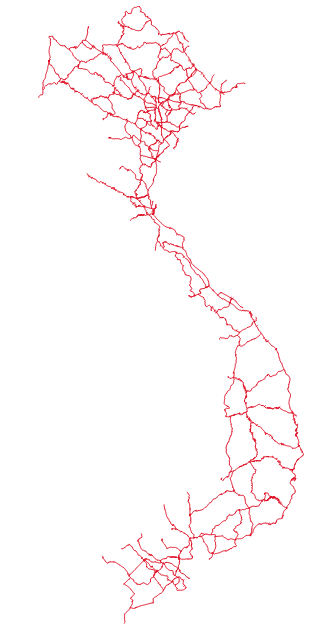
\includegraphics[width=0.5\textwidth]{figures/vietnamroad.png} % first figure itself
		\caption[dữ liệu đường bộ Việt Nam]{dữ liệu đường bộ Việt Nam, hiển thị bằng phần mềm QGIS.}
	\end{minipage}\hfill
	\begin{minipage}{0.6\textwidth}
		\centering
		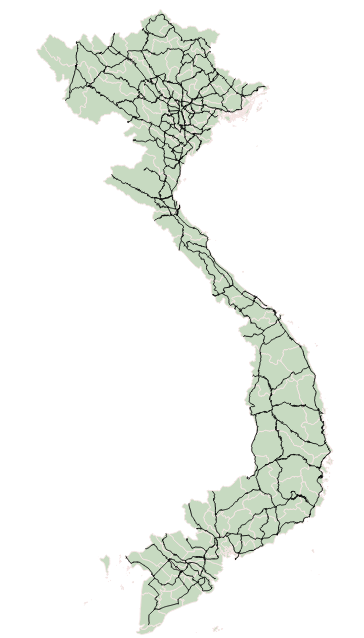
\includegraphics[width=0.5\textwidth]{figures/vietnamroad03.png} % second figure itself
		\caption[dữ liệu đường bộ Việt Nam được đặt trên bản đồ địa chính]{dữ liệu đường bộ Việt Nam được đặt trên bản đồ địa chính.}
	\end{minipage}
\end{figure}

\subsubsection{Phương pháp mô hình đồ thị cho dữ liệu GIS đường bộ Việt Nam}
Ban đầu khởi tạo đồ thị vô hướng rỗng $G$. Ánh xạ mỗi điểm đầu và điểm cuối của một đoạn đường với hai đỉnh tương ứng được thêm mới vào đồ thị $G$. Thêm một cạnh giữa hai đỉnh này vào đồ thị $G$, ứng với đoạn đường đó trên dữ liệu GIS. Các thuộc tính của đoạn đường trong dữ liệu GIS như tên, độ dài, mã code, được lưu như các thuộc tính của cạnh tương ứng trong đồ thị $G$.
Mỗi điểm trên đồ thị $G$ ứng với một đầu mút của một hay nhiều đoạn đường trên dữ liệu GIS.
Kết quả xử lý dữ liệu GIS để thu được đồ thị được biểu diễn trong hình 5. Các đỉnh của đồ thị được đặt vào các vị trí tương đối với nhau như trên địa lý.

\begin{figure}[!h]
	\centering
	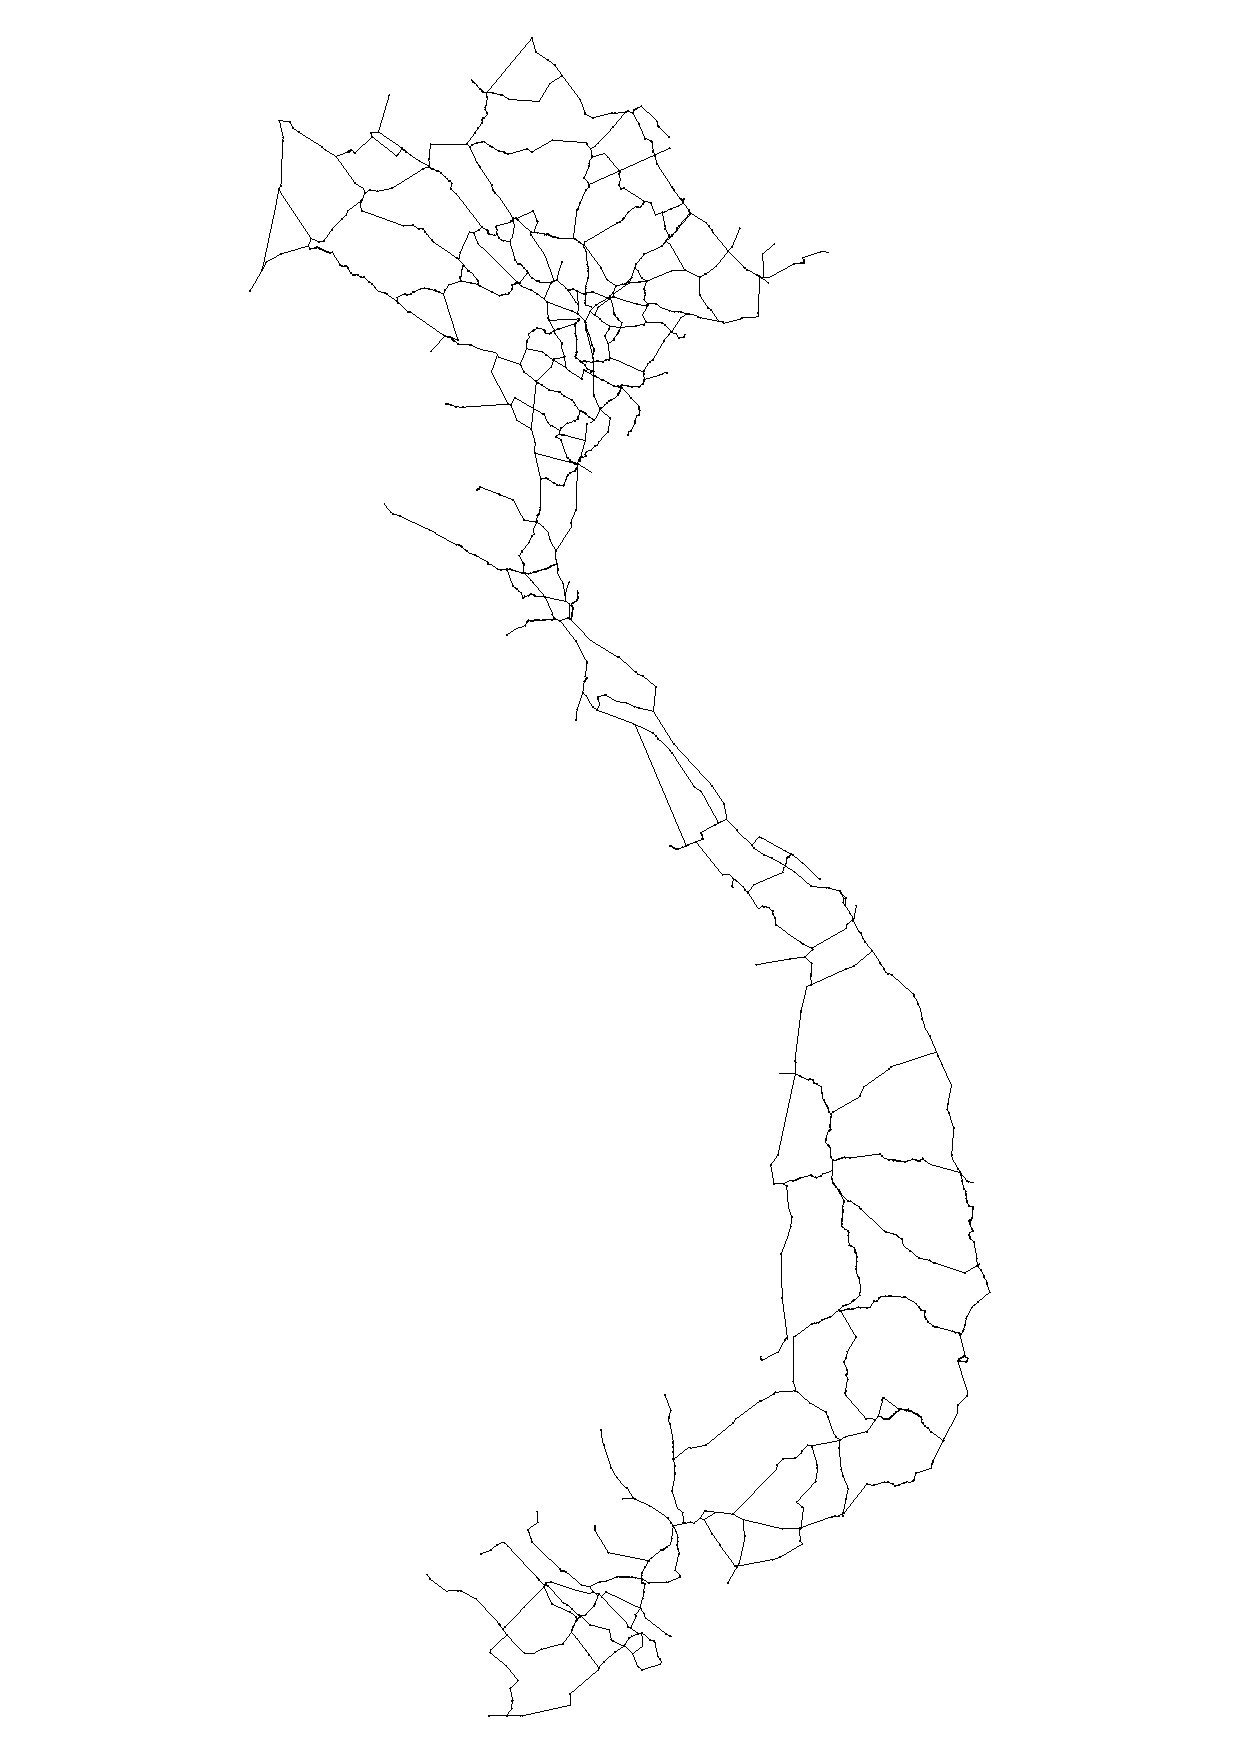
\includegraphics[scale=0.5]{figures/vietnamroad.pdf} 
	\caption[Đồ thị mạng đường bộ Việt Nam]{Đồ thị mạng đường bộ Việt Nam}
\end{figure}

\subsection{Những đặc trưng cơ bản trong phân tích đồ thị}
Một trong những bài toán trong phân tích đồ thị là quyết định độ quan trong của một đỉnh hay một cạnh. Chỉ số \textbf{tính trung tâm} \index{tính trung tâm} (centrality) của một đỉnh trong đồ thị thường chỉ ra mức độ ảnh hưởng của một đỉnh đó đến toàn bộ đồ thị. Có rất nhiều loại chỉ số trung tâm khác nhau và mỗi chỉ số có cách tính cũng như ý nghĩa khác nhau trong đánh giá độ quan trọng của một đỉnh và cạnh của đồ thị. Sau đây ta giới thiệu những chỉ số trung tâm cơ bản và ý nghĩa của chúng trong mạng giao thông.

\subsubsection{Khoảng cách, tâm sai, bán kính, đường kính của đồ thị}
Ta sẽ nhắc lại một số khái niệm cơ bản về lý thuyết đồ thị được sử dụng trong phần này.

\cite{graphtextbook} Cho đồ thị $G=(V,E)$, \textbf{khoảng cách} \index{khoảng cách} giữa hai đỉnh $u$ và $v$ của đồ thị $G$ là độ dài của đường đi ngắn nhất giữa hai đỉnh. Khoảng cách này kí hiệu là $d(u,v)$.

\cite{graphtextbook} \textbf{Tâm sai} \index{Tâm sai} (eccentricity) của một đỉnh trong một đồ thị liên thông là khoảng cách lớn nhất từ một đỉnh đến các đỉnh khác của đồ thị:
\begin{equation}
	\sigma(v) = \max_{u \in v} d(u,v)
\end{equation}

\cite{graphtextbook} Đường kính của đồ thị liên thông $G$, kí hiệu là $diam(G)$ là khoảng cách lớn nhất giữa hai đỉnh của đồ thị. Công thức tính đường kính của đồ thị:
\begin{equation}
	diam(G) = \max_{v \in V} \sigma(v)
\end{equation}

\cite{graphtextbook} Bán kính của đồ thị liên thông $G$ là giá trị nhỏ nhất của tâm sai của một đỉnh trong các đỉnh của đồ thị:
\begin{equation}
	rad(G) = \min_{v \in V} \sigma(v)
\end{equation}

\cite{graphtextbook} Mối quan hệ giữa bán kính và đường kính của đồ thị $G$:
\begin{equation}
	rad(G) \leq diam(G) \leq 2 * rad(G)
\end{equation}

\subsubsection{Hệ số phân cụm}
\begin{definition}
	\cite{complexnetwork}Cho đồ thị $G = (V,E)$, hệ số phân cụm \index{hệ số phân cụm} của một đỉnh $v \in V(G)$ kí hiệu là $cc(v)$ được định nghĩa là tỉ lệ giữa số cạnh tồn tại giữa các lân cận của đỉnh $v$ và số dạnh tối đa có thể có giữa những lân cận. Ta có công thức:
	\begin{equation}
		cc(v) = \frac{2m_v}{n_v(n_v-1)}
	\end{equation}
	trong đó $n_v$ là số đỉnh lân cận của đỉnh $v$ và $m_v$ là số cạnh giữa các lân cận của đỉnh $v$.
\end{definition}

Hệ số phân cụm $cc(v)$ trên được gọi là hệ số phân cụm địa phương. Hệ số phân cụm trung bình $CC(G)$ của đồ thị $G$ là trung bình giá trị của hệ số phân cụm của tất cả các đỉnh trong đồ thị:
\begin{equation}
	CC(G) = \frac{1}{n}\sum_{v \in V}cc(v)
\end{equation}
Một giá trị hệ số phân cụm trung bình thấp cho thấy tính liên kết kém giữa các cặp đỉnh của đồ thị. Nói cách khác, $CC(G)$ cho thấy độ dầy đặc của đồ thị.

Một phương pháp khác để tính hệ số phân cụm là sử dụng đồ thị tham giác và đồ thị bộ ba (triad). Đồ thị tam giác là đồ thị $K_3$, đồ thị bộ ba là đồ thị $P_3$. Ta có thể nhận thấy rằng số đồ thị tam giác mà một đỉnh kề với, chính là số cạnh giữa các đỉnh lân cận của đỉnh đó, số đồ thị bộ ba mà một đỉnh kề với, chính là số cạnh tối đa có thể có giữa các đỉnh lân cận của đỉnh đó.
Dựa trên điều này, ta có công thức khác tính hệ số phân cụm của một đỉnh:
\begin{equation}
	cc(v) = \frac{n_t(v)}{n_x(v)}
\end{equation}
với $n_t(v)$ và $n_x(v)$ lần lượt là số đồ thị tam giác và số đồ thị bộ ba ứng với đỉnh $v$ của đồ thị.

\begin{definition}
	\cite{complexnetwork} Cho một đồ thị đơn liên thông $G = (V,E)$ và $n_t(G)$ là số đồ thị tam giác phân biệt trong $G$, $n_t(G)$ là số đồ thị bộ ba phân biệt trong $G$. Hệ số bắc cầu \index{Hệ số bắc cầu} (network transitivity) của đồ thị $G$, $\tau(G)$ là tỉ lệ giữa $n_t(G)$ và $n_x(G)$, có công thức.
	\begin{equation}
		\tau(G) = \frac{3n_t(G)}{n_x(G)} = \frac{\sum n_t(v)}{\sum n_x(v)}
	\end{equation}
	Sở dĩ có số 3 trong công thức vì mỗi đỉnh của đồ thị tam giác được tính một lần trong $n_x(G)$.
\end{definition}

\begin{figure}[!h]
	\centering
	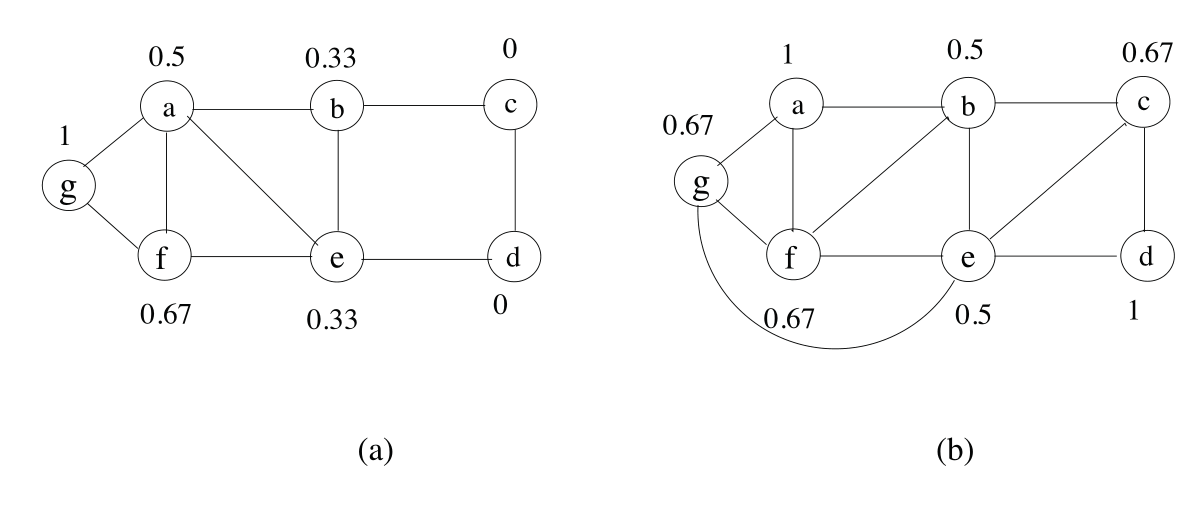
\includegraphics[scale=0.5]{figures/clustercoefficient.png} 
	\caption[Hệ số phân cụm]{Hệ số phân cụm của đồ thi (a) là 0.4 trong khi hệ số phân cụm của đồ thị (b) là 0.71, thể hiện rằng đồ thị (b) dày đặc hơn và có kết nối với nhau nhiều hơn.}
	\label{fig:clustercoeff}
\end{figure}

%\subsubsection{Những mô hình mạng}
%Những mô hình mạng đã được phân lớp rõ ràng: mạng ngẫu nhiên (random network), mạng thế giới nhỏ (small world network) và mạng không tỉ lệ (scale-free network).

%\begin{paragraph}
%	Mạng ngẫu nhiên, lần đầu tiên được đê xuất bởi Erdos và Renyi \cite{randnet} 
%\end{paragraph}

\subsubsection{Chỉ số trung tâm bậc và chỉ số trung tâm gần gũi}
Chỉ số trung tâm bậc (degree centrality) dựa trên ý tưởng rằng một đỉnh quan trọng thì có bậc hay số đỉnh kề với nó cao. Cho đồ thị $G=(V,E)$, $|V(G)| = N$, công thức chuẩn hóa của chỉ số trung tâm bậc của đỉnh $i$ trong đồ thị $G$, $C_D(i)$ được định nghĩa bởi Freeman \cite{centrali01},\cite{centrali02}:
\begin{equation}
	C_D(i) = \frac{k_i}{N-1} = \frac{\sum_{j \in N}a_{ij}}{N-1}
\end{equation}
trong đó $k_i$ là số cạnh $(i,j)$ nối đỉnh $i$ với các đỉnh khác của đồ thị, $a_{ij}$ là giá trị của ô $(i,j)$ trong ma trận kề biểu diễn cho đồ thị $G$.

Đối với đồ thị mạng giao thông (không kể đến mạng giao thông hàng không) thì chỉ số trung tâm bậc bị giới hạn bởi không gian, khi coi các đỉnh là các điểm nút giao thông, bậc của các đỉnh trong đồ thị này thường thấp (số lượng ngã 5, ngã 6 thường rất ít trong mạng giao thông thực tế).

Chỉ số trung tâm gần gũi (closeness centrality measure) được đề xuất bởi Sabidussi \cite{centrali03} là nghịch đảo của khoảng cách trung bình từ đỉnh i đến mọi đỉnh khác trong đồ thị, có công thức chuẩn hóa:
\begin{equation}
C_C(i) = \frac{N-1}{\sum_{j \in V} d(i,j)}
\end{equation}
trong đó $d(i,j)$ là khoảng cách giữa hai đỉnh $i$ và $j$.

Vì trong đồ thị, chỉ số trung tâm gần gũi phụ thuộc rất nhiều vào vị trí của đỉnh, đo đó trong mạng giao thông, các đỉnh ở vị trí trung tâm địa lý chắc chắn sẽ có chỉ số trung tâm gần gũi cao.

Chỉ số \textbf{trung tâm trung gian} \index{trung tâm trung gian} (betweeness centrality) của một đỉnh là số đường đinh ngắn nhất giữa tất cả các đỉnh mà có đi qua đỉnh đó \cite{centrali02}. Công thức của chỉ số trung tâm không gian được chuẩn hóa:
\begin{equation}
	C_B(i) = \frac{1}{(N-1)(N-2)} \sum_{j,k \in V(G); j \neq k; k\neq i; j \neq i} \frac{n_{jk}(i)}{n_{jk}}
\end{equation}
trong đó $n_{jk}$ là tổng số đường đi ngắn nhất giữa hai đỉnh $j$ và $k$, $n_{jk}(i)$ là số đường đi ngắn nhất giữa hai đỉnh $j$ và $k$ mà có đi qua đỉnh i.

Công thức $C_B(i)$ trên đã được chuẩn hóa và đạt giá trị cao nhất là 1 khi mọi đường đi ngắn nhất trong đồ thị đều chứa đỉnh $i$. Một định nghĩa tương tự chỉ số trung tâm trung gian cho cạnh cũng có thể được định nghĩa.

\subsubsection{Efficiency và straightness centrality}
Bắt nguồn từ ý tưởng rằng hiệu quả của một mạng không gian có thể được tính bằng việc so sánh độ dài của đường đi ngắn nhất giữa các đỉnh và khoảng cách chim bay giữa các đỉnh đó \cite{efficiency01}. Chỉ số trung tâm hiệu quả (efficiency centrality) $C_E(i)$ và chỉ số trung tâm thẳng (straightness centrality) $C_S(i)$ được định nghĩa \cite{efficiency02}:
\begin{equation}
C_S(i) = \frac{1}{N-1} \mathlarger{\sum}_{j \in V(G); j \neq i} \frac{d^{\text{crowfly}}(i,j)}{d(i,j)}
\end{equation}
\begin{equation}
	C_E(i) = \frac{\mathlarger{\sum}_{j \in V(G); j \neq i}\frac{1}{d(i,j)}}{\mathlarger{\sum}_{j \in V(G); j \neq i}\frac{1}{d^{\text{crowfly}}(i,j)}}
\end{equation}
trong đó $d^{\text{crowfly}}(i,j)$ là khoảng cách chim bay giữa hai đỉnh $i$,$j$ của mạng.

\subsection{Phân tích mạng đường bộ Việt Nam}
\newpage
\subsubsection{Phân tích các tham số cơ bản}
Hình \ref{fig:degreedist} biểu diễn biểu phân phối bậc của các đỉnh trong đồ thị mạng đường bộ Việt Nam.Trong dữ liệu GIS đường bộ Việt Nam có rất nhiều đoạn đường ngắn, nối tiếp nhau, của cùng một tên đường, nên ta có thể thấy là số đỉnh bậc 2 chiếm đa số trong phân phối bậc của đỉnh. Còn lại số đỉnh bậc 1,3 và 4 của đồ thị khá hợp lý, tương tự với kết quả thu được trong phân tích mạng giao thông của Thụy Sĩ \cite{swissroad}, số đỉnh bậc 3 chiếm đa phần nếu không tính các đỉnh bậc 2 sinh ra do dữ liệu chưa chuẩn.

Các 

\begin{figure}[!h]
	\centering
	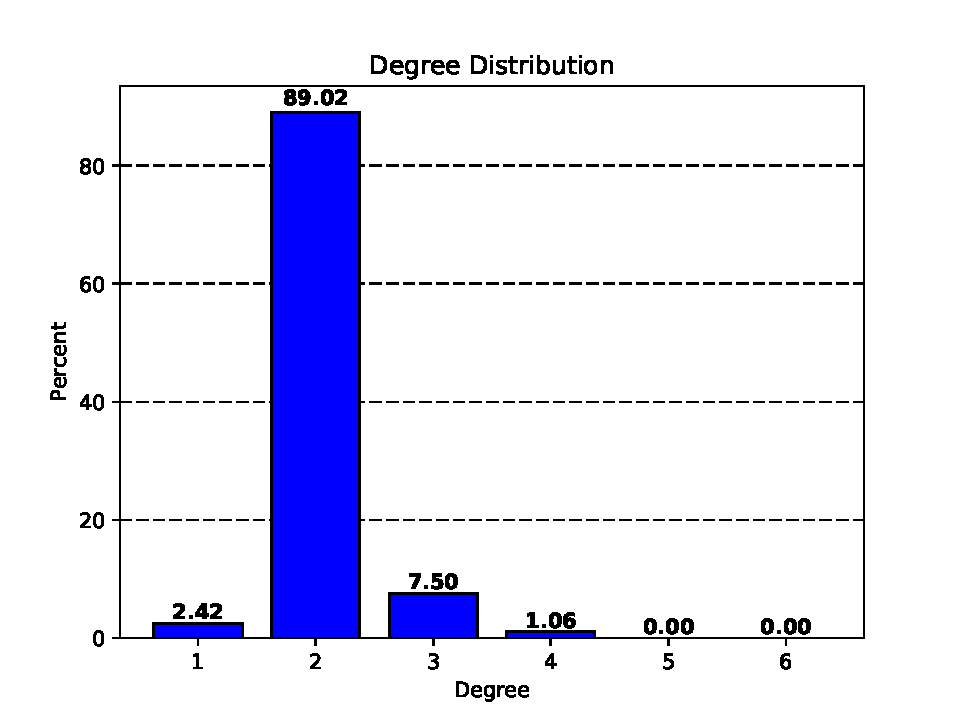
\includegraphics[scale=0.8]{figures/degreedist.pdf} 
	\caption[Phân phối bậc của đỉnh trong mạng đường bộ Việt Nam]{Phân phối bậc của đỉnh trong mạng đường bộ Việt Nam.}
	\label{fig:degreedist}
\end{figure}

\section{Kết luận}

%%%%%
\printindex
%%%%%
\newpage
\begin{thebibliography}{9}
	\bibitem{graphtextbook}
	Douglas B. West,
	\textit{Introduction to graph theory, Second Edition},
	Prentice Hall, ISBN: 9780130144003, 2001
	%
	\bibitem{yannakakis01}
	Yannakakis M.,
	"Node-Deletion Problems on Bipartite Graphs",
	SIAM Journal on Computing 10 (2 1981), pp. 310–327. ISSN: 0097-5397.
	%
	\bibitem{graphclasses}
	ISGCI: Information System on Graph Class Inclusions v2.0. "List of Small Graphs." \href{http://www.graphclasses.org/smallgraphs.html}{http://www.graphclasses.org/smallgraphs.html}.
	%
	\bibitem{swissroad}
	Alexander Erath, Michael Löchl, Kay W. Axhausen,
	"Graph-Theoretical Analysis of the Swiss Road and Railway Networks Over Time", 
	Networks and Spatial Economics,
	September 2009, Volume 9, Issue 3, pp 379–400
	%
	\bibitem{MIS}
	Ngoc C. Lê.
	"Algorithms for the Maximum Independent Set Problem",
	%
	\bibitem{MAXAlgorithm}
	Griggs, J. R.
	"Lower Bounds on the Independence Number in Terms of the Degrees",
	\textit{Combinatorica} 1 (2 1981), pp. 169–197.
	%
	\bibitem{VOAlgorithm}
	Mahadev, N. V. R. and Reed, B. A.
	"A Note on Vertex Order for Stability Number",
	\textit{Journal of Graph Theorey} 30 (2 1999), pp. 113–120.
	%
	\bibitem{alpharedundant}
	Brandstädt, A. and Hammer, P. L.
	\textit{"A Note on $\alpha$-redundant Vertices in Graphs"},
	Discrete Applied Mathematics 108 (3 2001), pp. 301–308.
	%
	\bibitem{alpharedudant2}
	Gerber, M. U. and Lozin, V. V.,
	"Robust Algorithms for the Stable Set Problem",
	Graphs and Combinatorics 19 (3 2003), pp. 347–356. ISSN: 1435-5914.
	%
	\bibitem{BasicEpid}
	R. Bonita, R. Beaglehole, Tord Kjellström,
	\textit{Basic epidemiology},
	World Health Organization 2009, second edition.
	%
	\bibitem{centrali01}
	Freeman, L.C.
	"Centrality in social networks: conceptual clarification",
	Social Networks, (1979) pp. 215-239.
	%
	\bibitem{centrali02}
	Freeman, L. C.
	"A set of measures of centrality based on betweenness",
	Sociometry, (1977) Vol. 40, No. 1, pp. 35-41.
	%
	\bibitem{centrali03}
	Sabidussi, G. 
	"The centrality index of a graph",
	 Psychometrika, Vol. 31 , pp. 581-603.
	 %
	 \bibitem{efficiency01}
	 Latora, V. and M. Marchiori,
	 "Efficient beahviour of small-world networks",
	 "Physical Review Letters" (2001), Vol. 87.
	 %
	 \bibitem{efficiency02}
	 Latora, V. and M. Marchiori, 
	 "Is the Boston subway a small-world network?",
	 Physica A (2002), Vol. 314 , pp. 109–113.
	 %
	 \bibitem{complexnetwork}
	 Kayhan Erciyes,
	 \textit{Complex Networks: An Algorithmic Perspective},
	 CRC Press, isbn: 1466571667, 9781466571662, 2014.
	 %
	 \bibitem{randnet}
	 P. Erdos andA. Renyi.
	 "On random graphs",
	 Publicationes Mathematicae, pp. 290-297, 1959.
\end{thebibliography}

\end{document}